\subsection*{Spherical Coordinate}
\paragraph{Introduction}


\paragraph{Geometrical model}

First, we are going to derive a general expression and after that apply it to a scenario with a drone and a basestation. In figure  \ref{fig:GeometricDist_general} the relationship between the height of the observer above sea level (O point) and the distance d which is between it and the horizon (H point) is shown. Finding this distance is done by the use of the pythagorean theorem. With some simple mathematical calculations the distance d is derived in the following:
\begin{align*}
&(R+h)^2 = R^2+d^2\nonumber \\
&\Rightarrow R^2+2hR+h^2 = R^2+d^2 \Rightarrow d^2 = 2hR + h^2 \\
&\Rightarrow d = \sqrt{2hR + h^2}\numberthis \label{eq:los_distToHorizon}
\end{align*} 

\begin{figure}%
    \centering
    \subfloat[Geometrical distance to the horizon]{{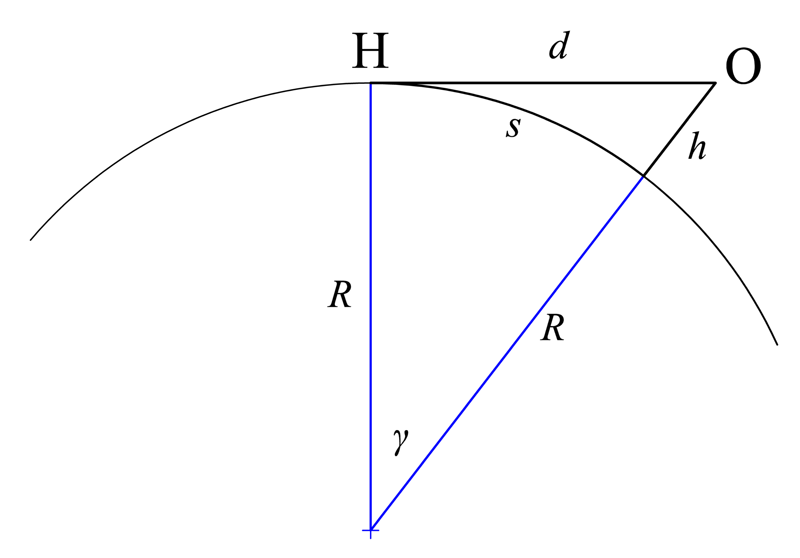
\includegraphics[width=6cm]{figures/GeometricDistanceToHorizonOneTriangle.png} 
\label{fig:GeometricDist_general}   }}%
    \qquad
    \subfloat[Geometrical distance from drone to basestation]{{
    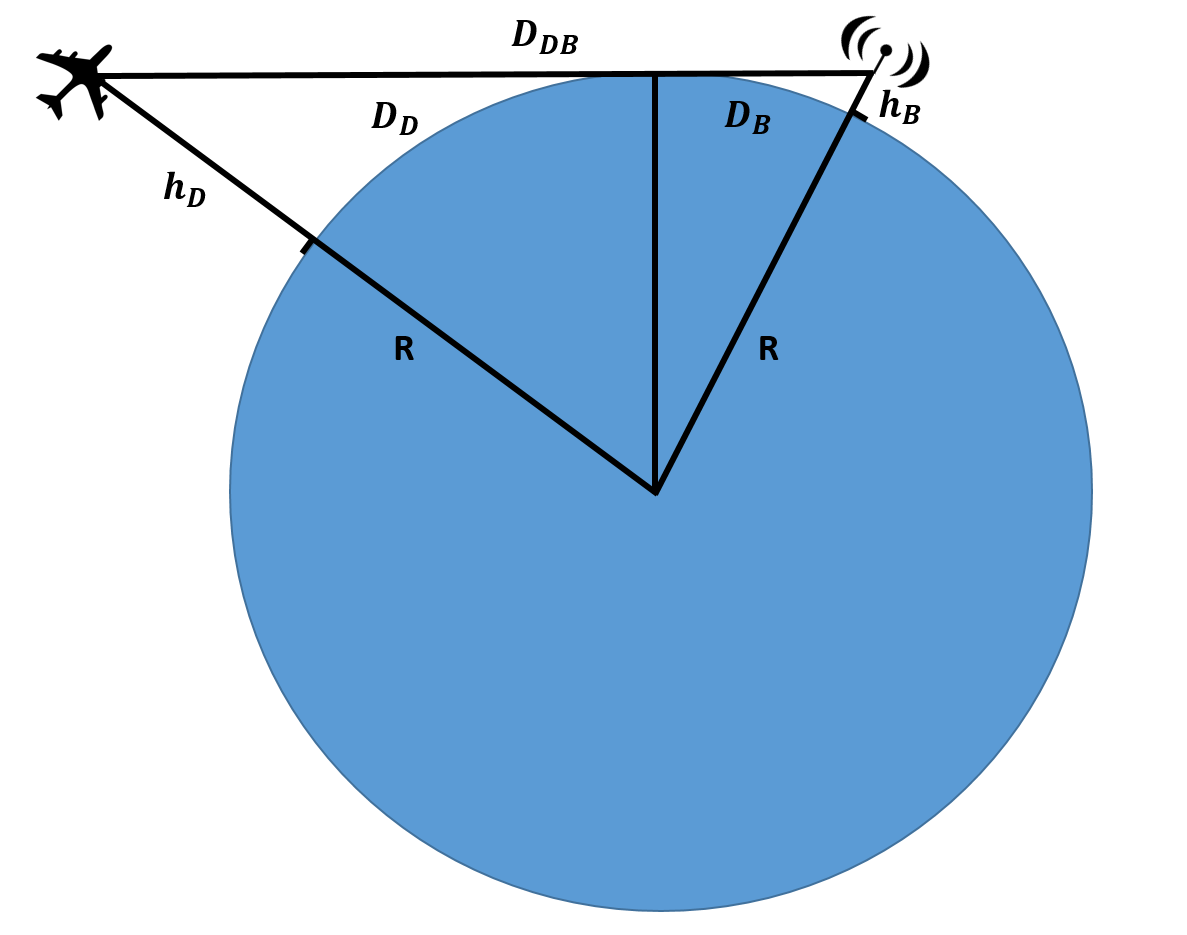
\includegraphics[width=6cm]{figures/GeometricDistanceToHorizonTwoTriangle.png} 
    \label{fig:GeometricDist_droneBasestation}  }}%
    \caption{Geometrical distance to the horizon, Pythahorean theorem}%
    \label{fig:GeometricDistanceToHorizon}%
\end{figure}
